\chapter{Combinational Circuit Building Blocks}\label{ch:blocks}

\begin{objectives}
After studying this chapter you will be able to:
\begin{itemize}
  \item analyse a given combinational circuit to find its Boolean functions, truth table and purpose, and follow a systematic procedure to design a new one;
  \item design a code converter, such as BCD to excess-3, and a decimal (BCD) adder;
  \item explain the operation of decoders, demultiplexers, encoders and priority encoders, and build larger ones from smaller ones;
  \item use a multiplexer to implement any Boolean function, and state Shannon's expansion theorem;
  \item describe the structure of a simple arithmetic logic unit (ALU);
  \item explain three-state gates and why buses need them; and
  \item design a magnitude comparator, and describe all of these blocks in VHDL.
\end{itemize}
\end{objectives}

\section{Combinational and Sequential Circuits}
Digital circuits are of two kinds. In a \term{combinational circuit} the outputs depend \emph{only on the present values of the inputs}: the circuit has no memory, and its behaviour is completely described by a truth table with $2^n$ rows for $n$ inputs. An adder is the typical example. In a \term{sequential circuit} the outputs depend on the inputs \emph{and on the state} held in memory elements (flip-flops), and therefore on past inputs; a counter is the typical example. Sequential circuits are the subject of Chapters~6--8.

The combinational circuits of this chapter are so frequently needed that they are provided as standard functions: as medium-scale-integration (MSI) chips in the 74xx series, as library cells, and as ready-made components in any HDL design tool. We study them in order to use them and to understand what a synthesis tool produces. \Cref{fig:comb-block} shows a combinational circuit as a block with $n$ inputs and $m$ outputs.

\figw{238.3pt}{lect_5_combinational_logic_circuit}{A combinational circuit has $n$ input variables and $m$ output variables.}{fig:comb-block}

\section{Analysis of a Combinational Circuit}\label{sec:analysis}
\termx{Analysis}{analysis} determines what function a given circuit implements.
\begin{enumerate}
  \item \textbf{Check that the circuit is combinational:} it must have no feedback paths and no memory elements.
  \item \textbf{Derive Boolean functions.} Label every gate output with a symbol; write the function at each gate output, starting at the inputs and working towards the outputs; then substitute to obtain the output functions in terms of the primary inputs only.
  \item \textbf{Make a truth table} by evaluating the output functions for all $2^n$ input combinations.
  \item \textbf{Explain the function} by observing the pattern in the truth table.
\end{enumerate}

\begin{example}{Analysis of a circuit}{analysis}
Analyse the circuit of \cref{fig:analysis-circuit}, which has inputs $A,B,C$ and outputs $F_1$, $F_2$.

\textbf{Solution.} Labelling the internal signals $T_1,T_2,T_3$ as in the figure:
\begin{align*}
 F_2 &= AB + AC + BC, & T_1 &= A+B+C, & T_2 &= ABC,\\
 T_3 &= F_2'\,T_1, & F_1 &= T_3 + T_2 .
\end{align*}
Substituting, $F_1 = (AB+AC+BC)'(A+B+C) + ABC$. The first term is 1 exactly when at least one input is 1 but fewer than two are (that is, exactly one input is 1), and $ABC$ covers the case where all three are 1. Hence
\[
 F_1 = A'B'C + A'BC' + AB'C' + ABC = A\xor B\xor C .
\]
The truth table (\cref{tab:analysis}) agrees: $F_1$ is the \emph{sum} bit and $F_2$ the \emph{carry} bit of $A+B+C$. The circuit is a \textbf{full adder}.
\end{example}

\begin{table}[htbp]
\centering
\caption{Truth table obtained in \cref{ex:analysis}.}
\label{tab:analysis}
\begin{tabular}{ccc|cc}
\toprule
$A$&$B$&$C$&$F_2$ (carry)&$F_1$ (sum)\\ \midrule
0&0&0&0&0\\0&0&1&0&1\\0&1&0&0&1\\0&1&1&1&0\\
1&0&0&0&1\\1&0&1&1&0\\1&1&0&1&0\\1&1&1&1&1\\ \bottomrule
\end{tabular}
\end{table}

\figw{375.6pt}{lect_5_analysis_example_circuit}{The circuit analysed in \cref{ex:analysis}.}{fig:analysis-circuit}

\section{Design Procedure}\label{sec:design}
\termx{Design}{design} is the inverse process: from a specification to a circuit.
\begin{enumerate}
  \item State the problem and understand the required behaviour.
  \item Determine the number of inputs and outputs; the inputs fix the truth-table size ($2^n$ rows).
  \item Assign symbols to the inputs ($A,B,C,\dots$ or $x,y,z,\dots$) and outputs ($F_1,F_2,\dots$).
  \item Derive the truth table.
  \item Derive and simplify the Boolean function of each output (K-maps or algebra).
  \item Draw the logic diagram (or write the HDL) and verify it by simulation.
\end{enumerate}

\subsection{Example: BCD to excess-3 converter}
The \term{excess-3 code} of a decimal digit is the 4-bit binary code of the digit plus 3; it is a self-complementing code used in some older decimal arithmetic circuits. We design a converter from BCD to excess-3.

\begin{example}{BCD to excess-3 code converter}{excess3}
\textbf{Steps 1--3.} The input is a BCD digit $ABCD$ ($A$ is the MSB) and the output is the excess-3 code $wxyz$ (\cref{fig:bcd-e3-block}). \textbf{Step 4.} Excess-3 is the BCD value plus 3 (\cref{tab:e3}); inputs 10--15 are not valid BCD and are don't-cares.

\textbf{Step 5.} The K-maps with don't-cares (\cref{fig:e3-kmaps}) give
\begin{align*}
 w &= A + BC + BD = A + B(C+D), & x &= B'C + B'D + BC'D' = B\xor(C+D),\\
 y &= CD + C'D' = (C\xor D)', & z &= D'.
\end{align*}
\textbf{Step 6.} The circuit is in \cref{fig:e3-circuit} and its VHDL description in \cref{lst:e3}. For $x$ we used the identity $B'(C+D)+B(C+D)'=B\xor(C+D)$.
\end{example}

\begin{table}[htbp]
\centering
\caption{BCD and excess-3 codes.}
\label{tab:e3}
\begin{tabular}{c|c|c}
\toprule
Decimal & BCD ($ABCD$) & Excess-3 ($wxyz$)\\ \midrule
0&0000&0011\\1&0001&0100\\2&0010&0101\\3&0011&0110\\4&0100&0111\\
5&0101&1000\\6&0110&1001\\7&0111&1010\\8&1000&1011\\9&1001&1100\\
10--15&1010--1111&xxxx\\ \bottomrule
\end{tabular}
\end{table}

\begin{figure}[htbp]
\centering
\begin{subfigure}[b]{167.5pt}\centering
  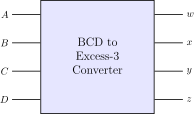
\includegraphics[width=165.5pt]{lect_5_bcd_to_excess3_block}\caption{block diagram}\label{fig:bcd-e3-block}
\end{subfigure}
\\[6pt]
\begin{subfigure}[b]{258.3pt}\centering
  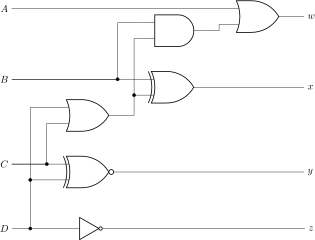
\includegraphics[width=256.3pt]{lect_5_bcd_to_excess3_circuit}\caption{logic diagram}\label{fig:e3-circuit}
\end{subfigure}
\caption{BCD to excess-3 converter of \cref{ex:excess3}.}
\end{figure}

\begin{figure}[htbp]
\centering
\begin{subfigure}[b]{382.0pt}\centering
  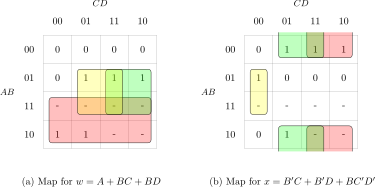
\includegraphics[width=380.0pt]{lect_5_bcd_kmaps_wx}\caption{K-maps for $w$ and $x$}
\end{subfigure}
\\[6pt]
\begin{subfigure}[b]{382.0pt}\centering
  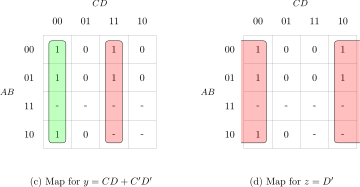
\includegraphics[width=380.0pt]{lect_5_bcd_kmaps_yz}\caption{K-maps for $y$ and $z$}
\end{subfigure}
\caption{K-maps for the outputs of the BCD to excess-3 converter; X marks don't-care inputs.}\label{fig:e3-kmaps}
\end{figure}

\vhdlfile{listings/ch05_bcd_to_excess3.vhd}{VHDL of the BCD to excess-3 converter.}{lst:e3}

\section{Decimal (BCD) Adder}\label{sec:bcdadder}
A \term{BCD adder} adds two BCD digits (plus a carry-in) and produces a BCD sum digit and a carry-out. A direct design would have 8 inputs (plus carry-in), a truth table with 256 rows and no usable K-map. A better idea is to reuse the 4-bit binary adder:
\begin{enumerate}
  \item add the two digits with a binary adder; the sum $Z$ (with carry $K$) lies between 0 and 19 ($9+9+1$);
  \item if the binary sum is 9 or less it is already the correct BCD digit;
  \item if it exceeds 9, add 6 ($\bin{0110}$): the extra 6 skips the six unused codes 10--15 and produces the correct decimal digit and a carry to the next decade.
\end{enumerate}
A correction is therefore needed if $K=1$ (sums 16--19) or if $Z\in\{10,\dots,15\}$ ($K=0$). In the latter range $Z_3=1$ always, and either $Z_2=1$ (12--15) or $Z_1=1$ (10, 11, 14, 15). The correction (and the carry-out) is
\begin{equation}
  C = K + Z_3Z_2 + Z_3Z_1 .
  \label{eq:bcdcorr}
\end{equation}
\Cref{fig:bcd-adder} shows the arrangement: the first adder forms $Z$, the logic of \cref{eq:bcdcorr} detects sums above 9, and the second adder adds $0110$ when $C=1$ and $0000$ otherwise.

\begin{example}{Adding BCD digits}{bcdadd}
$7+5$: the binary sum is $\bin{0111}+\bin{0101}=\bin{1100}=12>9$, so add $\bin{0110}$: $\bin{1100}+\bin{0110}=\bin{1\,0010}$. The carry is 1 and the digit is $\bin{0010}$: the BCD number $\bin{0001\,0010}=12$. \quad
$9+8+1$: $\bin{1001}+\bin{1000}+1=\bin{1\,0010}$, so $K=1$; adding 6 gives $\bin{1\,1000}$, the digit $\bin{1000}=8$ and carry 1, i.e.\ $18$.
\end{example}

\figw{206.8pt}{lect_5_bcd_adder}{A one-digit BCD adder: a binary adder, the correction-detection logic and a second adder that adds 6.}{fig:bcd-adder}

\vhdlfile{listings/ch05_bcd_adder.vhd}{Behavioural VHDL of a one-digit BCD adder. The package \code{numeric_std} provides the type \code{unsigned} and arithmetic on it.}{lst:bcdadder}

\section{Decoders}\label{sec:decoders}
A \term{decoder} converts binary information from $n$ input lines to at most $2^n$ unique output lines, so that for each input combination exactly one output is active. A decoder with $n$ inputs and $m\le2^n$ outputs is called an $n$-to-$m$-line decoder. \Cref{tab:dec38} gives the truth table of a 3-to-8 decoder, which is simply a generator of all eight \emph{minterms} of the three inputs: output $D_i$ is the minterm $m_i$. \Cref{fig:dec38} shows the block and its AND-gate implementation, and \cref{lst:dec} the VHDL.

\begin{table}[htbp]
\centering
\small
\caption{Truth table of a 3-to-8-line decoder (active-high outputs).}
\label{tab:dec38}
\begin{tabular}{ccc|cccccccc}
\toprule
$x$&$y$&$z$&$D_0$&$D_1$&$D_2$&$D_3$&$D_4$&$D_5$&$D_6$&$D_7$\\ \midrule
0&0&0&\textbf{1}&0&0&0&0&0&0&0\\
0&0&1&0&\textbf{1}&0&0&0&0&0&0\\
0&1&0&0&0&\textbf{1}&0&0&0&0&0\\
0&1&1&0&0&0&\textbf{1}&0&0&0&0\\
1&0&0&0&0&0&0&\textbf{1}&0&0&0\\
1&0&1&0&0&0&0&0&\textbf{1}&0&0\\
1&1&0&0&0&0&0&0&0&\textbf{1}&0\\
1&1&1&0&0&0&0&0&0&0&\textbf{1}\\ \bottomrule
\end{tabular}
\end{table}

\begin{figure}[htbp]
\centering
\begin{subfigure}[b]{169.5pt}\centering
  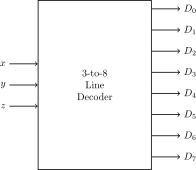
\includegraphics[width=167.5pt]{lect_5_decoder_3to8_block}\caption{block diagram}
\end{subfigure}
\hfill
\begin{subfigure}[b]{236.3pt}\centering
  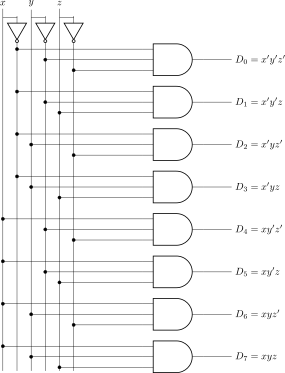
\includegraphics[width=234.3pt]{lect_5_decoder_3to8_circuit}\caption{logic diagram}
\end{subfigure}
\caption{A 3-to-8-line decoder.}\label{fig:dec38}
\end{figure}

\vhdlfile{listings/ch05_decoder_3to8.vhd}{A 3-to-8 decoder in VHDL.}{lst:dec}

\paragraph{Decoder with enable.} Decoders usually have an \term{enable} input $E$. In the common NAND-gate implementation of \cref{tab:dec-en} the outputs are active-low and the decoder works when $E=0$; when $E=1$ all outputs are inactive (1). \Cref{fig:dec-en} shows the circuit. Enable inputs allow decoders to be \emph{cascaded}: two 3-to-8 decoders form a 4-to-16 decoder if the most significant input drives the enable of one decoder directly and of the other through an inverter (\cref{fig:dec416}).

\begin{table}[htbp]
\centering
\scriptsize
\caption{3-to-8 decoder with active-low enable $E$ and active-low outputs.}
\label{tab:dec-en}
\begin{tabular}{c|ccc|cccccccc}
\toprule
$E$&$x$&$y$&$z$&$D_0$&$D_1$&$D_2$&$D_3$&$D_4$&$D_5$&$D_6$&$D_7$\\ \midrule
1&X&X&X&1&1&1&1&1&1&1&1\\
0&0&0&0&\textbf{0}&1&1&1&1&1&1&1\\
0&0&0&1&1&\textbf{0}&1&1&1&1&1&1\\
0&0&1&0&1&1&\textbf{0}&1&1&1&1&1\\
0&0&1&1&1&1&1&\textbf{0}&1&1&1&1\\
0&1&0&0&1&1&1&1&\textbf{0}&1&1&1\\
0&1&0&1&1&1&1&1&1&\textbf{0}&1&1\\
0&1&1&0&1&1&1&1&1&1&\textbf{0}&1\\
0&1&1&1&1&1&1&1&1&1&1&\textbf{0}\\ \bottomrule
\end{tabular}
\end{table}

\begin{figure}[htbp]
\centering
\begin{subfigure}[b]{229.3pt}\centering
  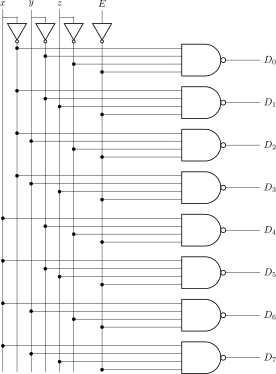
\includegraphics[width=227.3pt]{lect_5_decoder_3to8_enable_circuit}\caption{3-to-8 decoder with enable}\label{fig:dec-en}
\end{subfigure}
\caption{Decoder with enable input and cascading.}
\end{figure}

\begin{figure}[htbp]
\centering
\ContinuedFloat
\begin{subfigure}[b]{186.7pt}\centering
  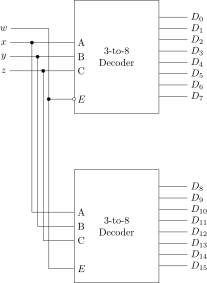
\includegraphics[width=184.7pt]{lect_5_decoder_4to16_block}\caption{4-to-16 decoder from two 3-to-8 decoders}\label{fig:dec416}
\end{subfigure}
\caption[]{Decoder with enable input and cascading.}
\end{figure}

\begin{keypoint}[Decoders implement functions]
Because the outputs of a decoder are the minterms of its inputs, any combinational function of $n$ variables can be implemented by an $n$-to-$2^n$ decoder and an OR gate that collects the minterms for which $f=1$. For example the full adder is $S=\Sm(1,2,4,7)$ and $C_{out}=\Sm(3,5,6,7)$: one 3-to-8 decoder and two 4-input OR gates.
\end{keypoint}

\subsection{Demultiplexers}
A \term{demultiplexer} (DEMUX) does the opposite of a multiplexer: it takes data from a single input line and routes it to one of $2^n$ output lines selected by $n$ select lines. A decoder with an enable input is a demultiplexer: the \emph{enable} becomes the \emph{data input} and the decoder inputs become the select inputs. \Cref{tab:demux} and \cref{fig:demux} show a 1-to-4 demultiplexer.

\begin{table}[htbp]
\centering
\caption{1-to-4 demultiplexer.}
\label{tab:demux}
\begin{tabular}{c|cc|cccc}
\toprule
Data&$S_1$&$S_0$&$Y_0$&$Y_1$&$Y_2$&$Y_3$\\ \midrule
$D$&0&0&$D$&0&0&0\\ $D$&0&1&0&$D$&0&0\\ $D$&1&0&0&0&$D$&0\\ $D$&1&1&0&0&0&$D$\\ \bottomrule
\end{tabular}
\end{table}

\figw{317.8pt}{lect_5_demux_1to4}{A 1-to-4 demultiplexer.}{fig:demux}

\section{Encoders}\label{sec:encoders}
An \term{encoder} performs the inverse of a decoder: it has $2^n$ (or fewer) input lines and $n$ output lines, and produces the binary code of the input line that is active. It is assumed that only one input is active at a time. For the octal-to-binary encoder with inputs $D_0,\dots,D_7$ and outputs $xyz$ (\cref{fig:enc83}),
\[
 x = D_4+D_5+D_6+D_7,\qquad y = D_2+D_3+D_6+D_7,\qquad z = D_1+D_3+D_5+D_7 .
\]
Each output is the OR of the inputs whose code has a 1 in that bit position. The simple encoder has two defects: the output is undefined if more than one input is active, and the all-zero output code is produced both by $D_0$ and by no input at all.

\figw{267.2pt}{lect_5_encoder_8to3_circuit}{An octal-to-binary (8-to-3) encoder.}{fig:enc83}

\subsection{Priority encoders}
A \term{priority encoder} gives each input a priority and outputs the code of the active input with the \emph{highest priority}. It also has a \emph{valid} output $V$ that shows whether any input is active, which resolves the second defect. \Cref{tab:prio} is the truth table of a 4-input priority encoder in which $D_3$ has the highest priority; X means don't-care. From it,
\[
 x = D_3 + D_2,\qquad y = D_3 + D_2'D_1,\qquad V = D_3+D_2+D_1+D_0 ,
\]
and \cref{fig:prio} is the circuit. Priority encoders are used, for example, to arbitrate interrupt requests.

\begin{table}[htbp]
\centering
\caption{4-to-2 priority encoder ($D_3$ has the highest priority).}
\label{tab:prio}
\begin{tabular}{cccc|ccc}
\toprule
$D_3$&$D_2$&$D_1$&$D_0$&$x$&$y$&$V$\\ \midrule
0&0&0&0&X&X&0\\0&0&0&1&0&0&1\\0&0&1&X&0&1&1\\0&1&X&X&1&0&1\\1&X&X&X&1&1&1\\ \bottomrule
\end{tabular}
\end{table}

\figw{237.0pt}{lect_5_priority_encoder_circuit}{A 4-to-2 priority encoder.}{fig:prio}

\section{Multiplexers}\label{sec:mux}
A \term{multiplexer} (MUX, or data selector) selects one of $2^n$ data inputs and connects it to a single output; $n$ \emph{select} lines determine which. We met the 2-to-1 multiplexer in \cref{ex:mux}. For the 4-to-1 multiplexer (\cref{tab:mux4}, \cref{fig:mux4}),
\[
 Y = S_1'S_0'I_0 + S_1'S_0I_1 + S_1S_0'I_2 + S_1S_0I_3 .
\]
\Cref{lst:mux-b} describes it behaviourally, as a selection (\code{when ... else}); \cref{lst:mux-s} gives the same function as a Boolean expression. Both produce the same hardware after synthesis, but the behavioural style is shorter and much easier to read and to scale to wider multiplexers.

\begin{table}[htbp]
\centering
\caption{4-to-1 multiplexer.}
\label{tab:mux4}
\begin{tabular}{cc|c}
\toprule $S_1$&$S_0$&$Y$\\ \midrule 0&0&$I_0$\\0&1&$I_1$\\1&0&$I_2$\\1&1&$I_3$\\ \bottomrule
\end{tabular}
\end{table}

\figw{262.8pt}{lect_5_mux_4to1_logic}{Logic diagram of a 4-to-1 multiplexer.}{fig:mux4}

\vhdlfile{listings/ch05_mux_4to1_behav.vhd}{4-to-1 multiplexer, behavioural architecture.}{lst:mux-b}
\vhdlfile{listings/ch05_mux_4to1_struct.vhd}{4-to-1 multiplexer written as a Boolean expression (``structural'' in the lecture notes).}{lst:mux-s}

\subsection{Implementing Boolean functions with multiplexers}
A multiplexer is a \emph{universal logic module}: any Boolean function of $n$ variables can be implemented by a multiplexer with $n-1$ select lines.
\begin{enumerate}
  \item Connect $n-1$ of the variables to the select inputs.
  \item Using an \emph{implementation table}, express $F$ for each select combination as a function of the remaining variable $D$. It is always one of $D$, $D'$, $0$ or $1$.
  \item Connect each data input $I_k$ to the corresponding $D$, $D'$, 0 or 1.
\end{enumerate}

\begin{example}{Function with an 8-to-1 multiplexer}{muxfunc}
Implement $F(A,B,C,D)=\Sm(1,3,4,11,12,13,14,15)$ with an 8-to-1 multiplexer.

\textbf{Solution.} Connect $A,B,C$ to the select inputs $S_2,S_1,S_0$. For each $ABC$ pair of rows, see where $F=1$ (\cref{tab:muximpl}). The data inputs are
\[
 I_0=D,\ I_1=D,\ I_2=D',\ I_3=0,\ I_4=0,\ I_5=D,\ I_6=1,\ I_7=1 .
\]
The circuit is \cref{fig:mux8}.
\end{example}

\begin{table}[htbp]
\centering
\small
\caption{Implementation table for \cref{ex:muxfunc}.}
\label{tab:muximpl}
\begin{tabular}{ccc|cc|c}
\toprule
$A$&$B$&$C$&$F$ for $D=0$&$F$ for $D=1$&Data input\\ \midrule
0&0&0&0&1&$I_0=D$\\
0&0&1&0&1&$I_1=D$\\
0&1&0&1&0&$I_2=D'$\\
0&1&1&0&0&$I_3=0$\\
1&0&0&0&0&$I_4=0$\\
1&0&1&0&1&$I_5=D$\\
1&1&0&1&1&$I_6=1$\\
1&1&1&1&1&$I_7=1$\\ \bottomrule
\end{tabular}
\end{table}

\figw{202.2pt}{lect_5_mux_8to1_func}{\Cref{ex:muxfunc}: a four-variable function with an 8-to-1 multiplexer.}{fig:mux8}

\subsection{Shannon's expansion theorem}
\term{Shannon's expansion theorem} states that any Boolean function can be split about any variable $x_i$:
\begin{equation}
  F(x_1,\dots,x_n) = x_i'\,F(x_1,\dots,0,\dots,x_n) + x_i\,F(x_1,\dots,1,\dots,x_n).
  \label{eq:shannon}
\end{equation}
The two terms are the \emph{cofactors} of $F$ with respect to $x_i$. Equation~\eqref{eq:shannon} is exactly the equation of a 2-to-1 multiplexer with select input $x_i$ and data inputs the two cofactors. Repeating the expansion for further variables gives a tree of 2-to-1 multiplexers: any $n$-variable function can be built from at most $2^{n-1}-1$ of them, with the last variable (or a constant) at the leaves.

\begin{example}{Multiplexer tree}{shannon}
Implement $F(A,B,C)=AB+C$ with 2-to-1 multiplexers.

\textbf{Solution.} Expanding on $A$: $F_{A'}=C$ and $F_A=B+C$. Expanding $F_A$ on $B$: $F_{AB'}=C$ and $F_{AB}=1$. Hence one multiplexer selected by $B$ with inputs $(C,1)$ produces $F_A$, and a second one selected by $A$ with inputs $(C, F_A)$ produces $F$ (\cref{fig:mux-tree}); two multiplexers suffice.
\end{example}

\figw{188.9pt}{lect_5_mux_tree_3var}{Multiplexer tree for a function of three variables.}{fig:mux-tree}

\section{The Arithmetic Logic Unit}\label{sec:alu}
An \term{arithmetic logic unit} (ALU) is a combinational circuit that performs a set of arithmetic and logic operations on two binary operands, the operation being chosen by select inputs. It is the computational core of every processor. A classic example is the 4-bit 74381 ALU (\cref{fig:alu-block}), which performs the eight operations of \cref{tab:alu} on operands $A$ and $B$ under the control of three inputs $S_2S_1S_0$. It also produces \emph{group propagate} and \emph{group generate} outputs, which serve as the inputs $P^*$ and $G^*$ of a carry-lookahead generator (\cref{sec:cla}), so that wider ALUs can be built without a long carry delay.

\begin{table}[htbp]
\centering
\caption{Function table of the 74381 ALU.}
\label{tab:alu}
\begin{tabular}{ccc|ll}
\toprule
$S_2$&$S_1$&$S_0$&Function&Operation\\ \midrule
0&0&0&Clear&$F=0000$\\
0&0&1&Subtract&$F=B-A$\\
0&1&0&Subtract&$F=A-B$\\
0&1&1&Add&$F=A+B$\\
1&0&0&XOR&$F=A\xor B$\\
1&0&1&OR&$F=A+B$ (logical)\\
1&1&0&AND&$F=A\cdot B$\\
1&1&1&Preset&$F=1111$\\ \bottomrule
\end{tabular}
\end{table}

Subtraction uses two's complement ($A+\NOT{B}+1$, \cref{sec:adders}). Each bit slice (\cref{fig:alu-slice}) contains a logic unit (AND, OR, XOR), an arithmetic unit (a full adder in propagate/generate form, $P_i=A_i\xor B_i$, $G_i=A_iB_i$) and a multiplexer, controlled by the select inputs, that chooses the result of the slice.

\begin{figure}[htbp]
\centering
\begin{subfigure}[b]{227.6pt}\centering
  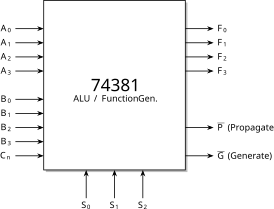
\includegraphics[width=225.6pt]{lect_5_alu_74381_block}\caption{block symbol}\label{fig:alu-block}
\end{subfigure}
\caption{The 74381 ALU: symbol and one bit slice.}
\end{figure}

\begin{figure}[htbp]
\centering
\ContinuedFloat
\begin{subfigure}[b]{412.0pt}\centering
  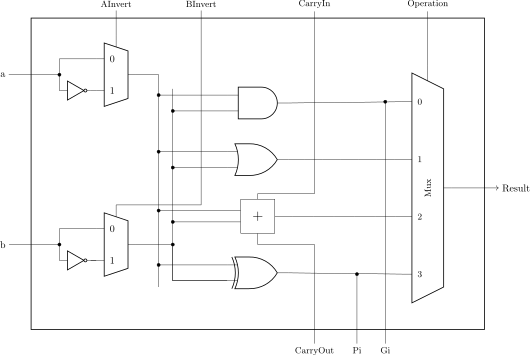
\includegraphics[width=410.0pt]{lect_5_alu_74381_logic}\caption{simplified 1-bit slice}\label{fig:alu-slice}
\end{subfigure}
\caption[]{The 74381 ALU: symbol and one bit slice.}
\end{figure}

\section{Three-State Gates and Buses}\label{sec:tristate}
A \term{three-state gate} (tri-state buffer) has three output states: logic 0, logic 1 and \term{high impedance} (Hi-Z), in which the output is effectively disconnected, like an open circuit. A control input $C$ selects the state: if $C=1$ the buffer is enabled and $\mathrm{Output}=\mathrm{Input}$; if $C=0$ the output is Hi-Z (\cref{fig:tristate}).

Three-state gates make it possible to connect several devices to a common wire, a \term{bus}, so long as \emph{only one device drives the bus at a time}. Two ordinary gates cannot drive the same wire: if one outputs 1 and the other 0 there is a low-resistance path between the supply and ground through the two output stages, a condition called \emph{bus contention} that causes a large current and an undefined voltage. \Cref{lst:tristate} shows the buffer in VHDL; the value \code{'Z'} of \code{std_logic} stands for high impedance. A three-state output can only be described behaviourally, because high impedance is a property of the output driver and cannot be formed from AND/OR/NOT gates.

\figw{147.7pt}{lect_5_tri_state_buffer}{A three-state buffer with enable input $C$.}{fig:tristate}

\vhdlfile{listings/ch05_tri_state_buffer.vhd}{A three-state buffer.}{lst:tristate}

\section{Magnitude Comparator}\label{sec:comparator}
A \term{magnitude comparator} compares two binary numbers $A$ and $B$ and produces three outputs: $A>B$, $A=B$ and $A<B$. The comparison proceeds from the most significant bit. Let $x_i = A_i\odot B_i = (A_i\xor B_i)'$ be 1 when the bits at position $i$ are equal. Then, for 4-bit numbers,
\begin{align*}
 (A=B) &= x_3x_2x_1x_0,\\
 (A>B) &= A_3B_3' + x_3A_2B_2' + x_3x_2A_1B_1' + x_3x_2x_1A_0B_0',\\
 (A<B) &= A_3'B_3 + x_3A_2'B_2 + x_3x_2A_1'B_1 + x_3x_2x_1A_0'B_0 .
\end{align*}
$A>B$ if at some position $A_i=1$, $B_i=0$ and all more significant bits are equal. The circuit is \cref{fig:comparator}; \cref{lst:comp-b,lst:comp-s} describe it behaviourally, and structurally with the equations above.

\figw{410.0pt}{lect_5_magnitude_comparator}{A 4-bit magnitude comparator.}{fig:comparator}

\vhdlfile{listings/ch05_magnitude_comparator_behav.vhd}{Behavioural description of the comparator using the relational operators.}{lst:comp-b}
\vhdlfile{listings/ch05_magnitude_comparator_struct.vhd}{Gate-level description of the comparator.}{lst:comp-s}

\begin{chaptersummary}
\begin{itemize}
  \item A \textbf{combinational circuit} has no memory. \textbf{Analysis}: label gate outputs, derive functions, build the truth table, explain. \textbf{Design}: specification, truth table, simplification, logic diagram, verification.
  \item \textbf{Code converters} such as BCD to excess-3 are designed with K-maps and don't-cares. The \textbf{BCD adder} adds 6 to a binary sum greater than 9, with $C=K+Z_3Z_2+Z_3Z_1$.
  \item A \textbf{decoder} generates the minterms of its inputs; with an enable input it is also a \textbf{demultiplexer} and can be cascaded. Any function can be built from a decoder and an OR gate.
  \item An \textbf{encoder} produces the code of the active input; a \textbf{priority encoder} handles several active inputs and has a valid output.
  \item A \textbf{multiplexer} selects one of $2^n$ inputs; it implements any function of $n+1$ variables, and Shannon's expansion gives a tree of 2-to-1 multiplexers.
  \item An \textbf{ALU} selects among arithmetic and logic operations; its group $P$ and $G$ outputs permit fast wide ALUs.
  \item \textbf{Three-state gates} (Hi-Z) allow many drivers on one bus, provided only one is enabled at a time.
  \item A \textbf{magnitude comparator} compares from the MSB downward using $x_i=A_i\odot B_i$.
\end{itemize}
\end{chaptersummary}

\chapsec{Exercises}
\begin{exlist}
  \item \textbf{Multiplexer expansion.} Construct a 4-to-1 multiplexer using only 2-to-1 multiplexers. How many are needed? \emph{Hint:} use the LSB select line $S_0$ in the first stage to choose within the pairs $(I_0,I_1)$ and $(I_2,I_3)$, and the MSB $S_1$ in the second stage.
  \item \textbf{Function with a 4-to-1 multiplexer.} Implement $F(A,B,C)=\Sm(1,3,5,6,7)$ with a single 4-to-1 multiplexer. Connect $A$ and $B$ to the select lines and find $I_0,\dots,I_3$ in terms of $C$.
  \item \textbf{Tri-state bus.} Explain why the outputs of two ordinary AND gates cannot be connected together to the same wire. What happens if one gate outputs 1 and the other 0? How does a three-state buffer solve the problem?
  \item \textbf{Comparator analysis.} For $A=\bin{1011}$ and $B=\bin{1001}$, find the equivalence signals $x_3,x_2,x_1,x_0$ and the outputs $A>B$, $A=B$, $A<B$.
  \item Analyse the circuit defined by $T_1=AB'$, $T_2=A'B$, $F=T_1+T_2+C$. Write $F$ as a function of $A,B,C$, make the truth table and describe the function in words.
  \item Implement the full adder ($S$ and $C_{out}$) with a 3-to-8 decoder (active-high outputs) and OR gates.
  \item Design a 4-to-2 priority encoder in which $D_0$ has the \emph{highest} priority and $D_3$ the lowest. Give the equations for $x$, $y$ and $V$.
  \item Implement $F(A,B,C,D)=\Sm(0,2,6,7,8,10,13,15)$ with an 8-to-1 multiplexer, using $A,B,C$ as the select inputs. Give the data inputs in terms of $D$.
  \item Implement $F=xy+x'z$ with a single 2-to-1 multiplexer. Identify the select and data inputs.
  \item Show how to build a 5-to-32 decoder from 3-to-8 decoders with enable inputs and one 2-to-4 decoder. How many of each are needed?
  \item How many 2-to-1 multiplexers are needed to build an 8-to-1 multiplexer?
  \item Add the BCD digits (a)~$\bin{0111}+\bin{0101}$ and (b)~$\bin{1001}+\bin{1001}+1$ using the BCD adder method, giving the binary sum, the correction and the result.
  \item Design a 2-bit magnitude comparator with outputs $A>B$, $A=B$, $A<B$ and draw the logic diagram. \emph{Hint:} $A>B = A_1B_1' + (A_1\odot B_1)A_0B_0'$.
  \item Design a combinational circuit that converts a 4-bit \emph{binary} number in the range 0--9 into the corresponding Gray code of that number, ($g_3=b_3$, $g_2=b_3\xor b_2$, $g_1=b_2\xor b_1$, $g_0=b_1\xor b_0$). Write its VHDL in one architecture with four concurrent assignments.
  \item A three-state buffer drives the bus with the value of an 8-bit register when the signal \code{rd} is 1. Write the VHDL, using a \code{std_logic_vector} of width 8 and the value \code{(others => 'Z')}.
\end{exlist}

\chapsec{Further Reading}
All the blocks of this chapter are treated in Chapter~4 of Mano and Ciletti~\cite{mano2018} and in Chapters~6 and~7 of Brown and Vranesic~\cite{brown2009}, including the VHDL descriptions; Wakerly~\cite{wakerly2006} also discusses MSI parts in detail. Ashenden~\cite{ashenden2008} is a good reference for the VHDL features used in the listings.
